\chapter{LTE}\label{lte}
Mobile communications is on to its fourth generation of network infrastructure with \ac{lte} (Long Term Evolution) (\ac{4g}). This network infrastructure is an improvement upon Universal Mobile Telecommunications System (\ac{umts}), which is a third generation network (\ac{3g}). LTE has downlink (\ac{dl}) speeds of up to 300 Mbit/s and uplink (\ac{ul}) speeds of 75 Mbit/s. This development was driven by the users want of faster download speeds for mobile services such as Video Streaming.
\section{Self Organising Network}\label{self organising network}
\ac{son}~\cite{feng2008self}
\section{Handover Procedure}\label{handover procedure}
\ac{ue} \ac{enodeb} \ac{mme}
\subsection{Handover Parameters}\label{handover parameters}
\ac{ttt} \ac{hys}

\begin{table}[H]
  \begin{center}
    \begin{tabular}{| l | p{2cm} |}
  	  \hline
      Parameter & Value(dB) \\ \hline
      hys & 0.0 \newline
      0.0 \newline
	  0.5 \newline
	  1.0 \newline
	  1.5 \newline
	  2.0 \newline
	  2.5 \newline
	  3.0 \newline
	  3.5 \newline
	  4.0 \newline
	  4.5 \newline
	  5.0 \newline
	  5.5 \newline
	  6.0 \newline
	  6.5 \newline
	  7.0 \newline
	  7.5 \newline
	  8.0 \newline
	  8.5 \newline
	  9.0 \newline
	  9.5 \newline	  	  	  	  
	  10.0 \\
      \hline
  	\end{tabular}
  \end{center}
  \caption{Table of the different LTE hys values.}
  \label{tab:hys}
\end{table}

\begin{table}[H]
  \begin{center}
    \begin{tabular}{| l | p{1.5cm} |}
  	  \hline
      Parameter & Value(s) \\ \hline
      TTT & 0.0 \newline
      0.04 \newline
	  0.064 \newline
	  0.08 \newline
	  0.1 \newline
	  0.128 \newline
	  0.16 \newline
	  0.256 \newline
	  0.32 \newline
	  0.48 \newline
	  0.512 \newline
	  0.64 \newline
	  1.024 \newline
	  1.280 \newline
	  2.56 \newline
	  5.12 \\
      \hline
  	\end{tabular}
  \end{center}
  \caption{Table of the different LTE TTT values.}
  \label{tab:ttt}
\end{table}

\begin{figure}[H]
  \begin{center}
    	  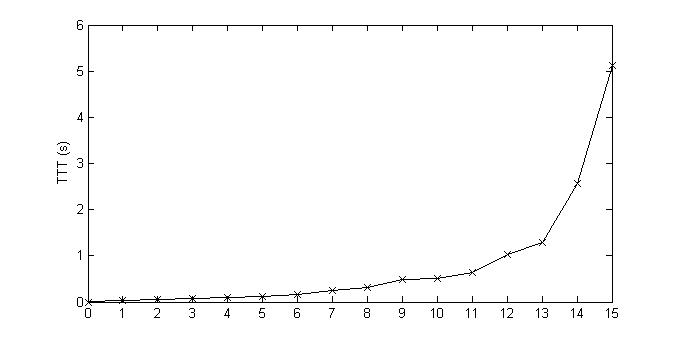
\includegraphics[width=0.5\textwidth]{figures/TTTgraph.jpg}
    \end{center}
    \caption{Graph of TTT values.}
    \label{fig:ttt}
\end{figure}

\subsection{Handover Triggers}\label{handover triggers}
\begin{table}[H]
  \begin{center}
    \begin{tabular}{| l | p{11.1cm} |}
  	  \hline
      Event Type & Trigger Criteria \\ \hline
      A1 & Serving becomes better than a threshold. \\
      A2 & Serving becomes worse than a threshold. \\
      A3 & Neighbour becomes offset better than PCell. \\
      A4 & Neighbour becomes better than threshold. \\
      A5 & PCell becomes worse than threshold1 and neighbour becomes better than threshold2. \\
      A6 & Neighbour becomes offset better than SCell. \\
      B1 & Inter RAT neighbour becomes better than threshold. \\
      B2 & PCell becomes worse than threshold1 and inter RAT neighbour becomes better than threshold2. \\
      \hline
  	\end{tabular}
  \end{center}
  \caption{Table of the different LTE Trigger types and their criteria.}
  \label{tab:trigger}
\end{table}

~\cite{3gpp2012proto}
~\cite{cox2012introduction}